%\section{Модели сложного теплообмена}\label{sec:$p_1$}
%
%\subsection{Стационарная модель}\label{subsec:st}
%\begin{frame}
%    \frametitle{Стационарная модель}
%    Область $\Omega \subset \mathbb{R}^3$, граница  $\Gamma = \partial \Omega$.
%    \begin{gather}
%        -a \Delta \theta + + b \kappa_a \theta^4 =  b \kappa_a \varphi,
%        \quad
%        - \alpha \Delta \varphi + \kappa_a \varphi = \kappa_a \theta^4,  \label{eq:pres:1}\\
%        a \frac{\partial \theta}{\partial \mathbf{n}}
%        +\left.\beta\left(\theta-\theta_{b}\right)\right|_{\Gamma}=0,
%        \quad
%        \alpha \frac{\partial \varphi}{\partial \mathbf{n}} + \gamma
%        (\varphi-\theta_b^4)|_{\Gamma} = 0. \label{eq:pres:2}
%    \end{gather}
%
%    Здесь $\theta$ -- нормализованная температура, $\varphi$ -- нормализованная интенсивность излучения,
%    усреднённая по всем направлениям, $\kappa_a$ -- коэффициент поглощения.
%    Константы $a, b, \alpha, \gamma, \beta$ описываются следующим образом:
%    \[
%        a = \frac{k}{\rho c_v}, \; b = \frac{4 \sigma n^2 T^3_{\max}}{\rho c_v}, \;
%        \alpha = \frac{1}{3\kappa -A \kappa_s},
%    \]
%
%
%
%    $\Omega$ -- липшицева ограниченная область, $\Gamma$ состоит из конечного числа гладких кусков,
%    исходные данные удовлетворяют условиям:
%    \begin{itemize}
%        \item (i) $\theta_{0}, \beta, \gamma \in L^{\infty}(\Gamma),
%        0 \leqslant \theta_{0} \leqslant M, \beta \geqslant \beta_{0}>0, \gamma \geqslant \gamma_{0}>0$;
%    \end{itemize}
%    Здесь $M, \beta_{0}, \gamma_{0}$, и $c_{0}$ положительные постоянные.
%\end{frame}
%\note{
%    Результаты, приведённые ниже служат теоретической основой для представленных
%    в диссертации алгоритмов обратных задач.
%
%    где $k$ -- теплопроводность, $c_v$ -- удельная теплоёмкость, $\rho$ -- плотность,
%    $\sigma$ -- постоянная Стефана\,--\,Больцмана, $n$ -- индекс рефракции,
%    $T_{\max}$ -- максимальная температура,
%    $\kappa \coloneqq \kappa_s + \kappa_a$ -- коэффициент полного взаимодействия,
%    $\kappa_s$ -- коэффициент рассеяния.
%    Коэффициент $A \in [-1,1]$ описывает анизотропию рассеивания;
%    случай $A=0$ отвечает изотропному рассеиванию.
%
%
%    Данная модель активно исследовалась моим научным руководителем А.Ю. Чеботарёвым,
%    в 2015г. было доказано существование и единственность решения для данной модели.
%
%    Этот результат удалось обобщить для квазистационарного и квазилинейного случая.
%    Об этом далее.
%}
%\begin{frame}
%    \frametitle{Алгоритм решения краевых задач}
%    \begin{itemize}
%        \item Линеаризация задачи методом Ньютона.
%        \item Триангуляция рассматриваемой области.
%        \item Применение метода конечных элементов для решения системы~\eqref{eq:pres:1}--\eqref{eq:pres:2}.
%    \end{itemize}
%    Линеаризация методом Ньютона:
%    \begin{equation}
%        \tag{L1}
%        \label{eq:L1}
%        \begin{gathered}
%            -a \Delta \theta+b \kappa_{a}\left(\left(4 \widetilde{\theta}^{3}
%            \theta-3 \widetilde{\theta}^{4}\right)-\varphi\right)=0,
%            \quad-\alpha \Delta \varphi
%            +\kappa_{a}\left(\varphi
%            -\left(4 \widetilde{\theta}^{3}
%            \theta-3 \widetilde{\theta}^{4}\right)\right)=0;
%        \end{gathered}
%    \end{equation}
%
%    \textbf{Пример}.
%    Пусть $\Omega=\{(x,y,z),\, 0 \leq x,y,z \leq 1 \}$.
%    Определим функции $\gamma, \theta_b$ следующим образом:
%    $\gamma = 0.8 \cos\left(\frac{\pi}{2} z\right) + 0.5$,
%    $\theta_b = 1- y / 2 + z /2$.
%
%    \begin{figure}[h!t]
%        \begin{minipage}[b][][b]{0.49\linewidth}
%            \centering
%            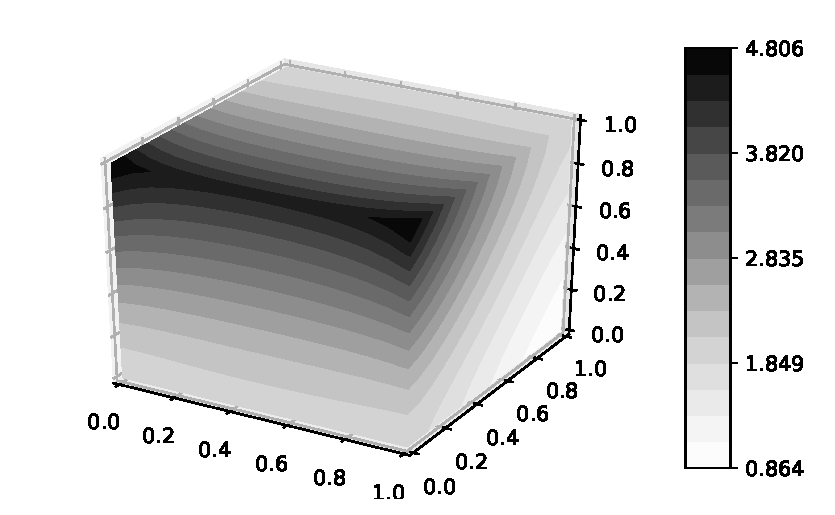
\includegraphics[width=1\linewidth]{boundary/theta_3d} \\ а) $\theta$
%        \end{minipage}
%        \hfill
%        \begin{minipage}[b][][b]{0.49\linewidth}
%            \centering
%            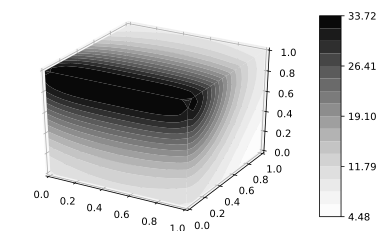
\includegraphics[width=1\linewidth]{boundary/phi_3d} \\ б) $\varphi$
%        \end{minipage}
%        \label{fig:4_1:boundary_3d}
%    \end{figure}
%\end{frame}
%\note{
%    Линеаризируем её методом Ньютона.
%    (Существенно улучшает сходимость алгоритмов!!
%    Что важно при решении задач типа Коши и др.)
%
%    Начальное приближение выберем нулевым.
%    Для нахождения состояния потребовалось шесть итераций,
%    результат представлен на рисунке.
%
%
%    Предложенный в работе алгоритм и программа решения краевых задач позволяет
%    уверенно рассчитывать температурное поле и поле излучения для произвольных областей.
%}
%
%\subsection{Квазистационарная модель}\label{subsec:qst}
%\begin{frame}
%    \frametitle{Квазистационарная модель}
%    \begin{align}
%        \frac{\partial\theta}{\partial t} - a\Delta\theta
%        + b\kappa_a (|\theta|\theta^3 - \phi) &= 0, \label{eq:1_5:1}\\
%        - \alpha\Delta\phi + \kappa_a (\phi - |\theta|\theta^3 ) &= 0,
%        \quad x \in \Omega, \quad 0 < t < T ; \label{eq:1_5:1+} \\
%        a \frac{\partial \theta}{\partial n}
%        +\left.\beta\left(\theta-\theta_{b}\right)\right|_{\Gamma}&=0,
%        \quad \alpha \frac{\partial \varphi}{\partial \mathbf{n}} + \gamma
%        (\varphi-\theta_b^4)|_{\Gamma} = 0 \text{ на } \Gamma; \label{eq:1_5:2} \\
%        \theta|_{t=0} &= \theta_0. \label{eq:1_5:3}
%    \end{align}
%    Предполагаем, что
%    \begin {itemize}
%        \item (j) $a, b, \alpha, \kappa_{a} =$ Const $>0$,
%        \item (jj) $\theta_{b}, q_{b}, u=\theta^4_b \in U, r
%        =a\left(\theta_{b}+q_{b}\right) \in L^{5}(\Sigma), \; \theta_{0} \in L^{5}(\Omega)$.
%    \end{itemize}
%
%    Здесь $\Sigma = \Gamma \times (0, T)$, $U$ -- пространство $L^{2}(\Sigma)$.
%
%    \begin{lemma}[1.20]
%        Пусть выполняются условия (j), (jj).
%        Тогда существует единственное слабое решение задачи~\eqref{eq:1_5:1}--\eqref{eq:1_5:3} и справедливо
%        \[
%            \psi=[\theta]^{5 / 2} \in L^{\infty}(0, T ; H) \cap L^{2}(0, T ; V),
%            \quad[\theta]^{4} \in L^{2}(0, T ; H).
%        \]
%    \end{lemma}
%\end{frame}
%\note{
%    Квазистационарная модель
%    Квазистационарная модель -- медленные изменения со временем или
%    имеющую относительно длительный период стабильности по сравнению с
%    интересующим масштабом времени.
%    Такие модели часто используются, когда
%    изучаемая система находится в равновесии или близка к нему, но при этом мо
%    жет испытывать небольшие, медленные колебания со временем.
%    Термин ‘квази‘ означает, что система не совсем стационарна,
%    ее состояние меняется настолько медленно,
%    его можно считать почти стационарным для определенных анализов или целей.
%
%    В контексте теплообмена, излучения или других физических процессов
%    квазистационарные модели могут использоваться для описания сценариев, ко
%    гда параметры и свойства системы меняются очень медленно по сравнению с
%    масштабом времени конкретного изучаемого явления.
%    Такие модели могут упростить анализ и снизить вычислительную сложность, позволяя исследователям
%    сосредоточиться на основных аспектах проблемы.
%
%    [Лемма] -- теоретический результат является новым и используется для обоснования
%    корректности оптимизационного метода для квазистационарной модели с данными Коши.
%}
%
%\subsection{Квазилинейная модель}\label{subsec:ql}
%\begin{frame}
%    \frametitle{Квазилинейная модель}
%    \begin{gather}
%        \sigma \partial \theta / \partial t
%        -\operatorname{div}(k(\theta) \nabla \theta)
%        +b\left(\theta^{3}|\theta|-\varphi\right)=f, \label{eq:1_6:1}\\
%        -\operatorname{div}(\alpha \nabla \varphi)
%        +\beta\left(\varphi-\theta^{3}|\theta|\right)=g, x \in \Omega, 0<t<T, \label{eq:1_6:2}\\
%        k(\theta) \partial_{n} \theta+\left.p\left(\theta-\theta_{b}\right)\right|_{\Gamma}=0,
%        \alpha \partial_{n} \varphi
%        +\left.\gamma\left(\varphi-\theta_{b}^{4}\right)\right|_{\Gamma}=0,
%        \left.\quad \theta\right|_{t=0}=\theta_{in}.\label{eq:1_6:3}
%    \end{gather}
%
%    Предполагаем, что:
%    \begin{itemize}
%        \item (k1) $\alpha, \beta, \sigma \in L^{\infty}(\Omega),
%        \quad b=r \beta, r = Const > 0; \alpha \geq \alpha_{0}, \beta \geq \beta_{0},
%        \sigma \geq \sigma_{0}, \alpha_{0}, \beta_{0}, \sigma_{0}=$ Const $>0$.
%
%        \item (k2) $0<k_{0} \leq k(s) \leq k_{1},\left|k^{\prime}(s)\right| \leq k_{2},
%        s \in \mathbb{R}, \quad k_{j}=$ Const.
%
%        \item (k3) $0 \leq \theta_{b} \in L^{\infty}(\Sigma), 0 \leq \theta_{\text{in}}
%        \in L^{\infty}(\Omega)$; $\gamma_{0} \leq \gamma \in L^{\infty}(\Gamma), p_{0}
%        \leq p \in L^{\infty}(\Gamma), \gamma_{0}, p_{0}=$ Const $>0$.
%
%        \item (k4) $0 \leq f, g \in L^{\infty}(Q).$
%    \end{itemize}
%
%
%    \begin{theorem}[1.7]
%        \label{th:1_6:1}
%        Если выполнены условия (k1)--(k4), то существует хотя бы одно
%        решение задачи~\eqref{eq:1_6:1}--\eqref{eq:1_6:3}.
%    \end{theorem}
%    \begin{theorem}[1.8]
%        Если выполнены условия (k1)--(k4) и $\theta_{*}, \varphi_{*}$ является
%        решением задачи~\eqref{eq:1_6:1}--\eqref{eq:1_6:3}
%        так, что $\theta_{*}, \nabla \theta_{*} \in L^{\infty}(Q)$,
%        то других ограниченных решений этой задачи нет.
%    \end{theorem}
%\end{frame}
%\note{
%    Зависимость коэффициента теплопроводности от температуры,
%    $\sigma$ – произведение удельной теплоемкости на объемную плотность (кг на м3),
%    f и g описывают вклад источников тепла и излучения соответственно.
%    Положительные параметры ... описывают радиационные и теплофизические свойства среды.
%
%    Свойства модели, установленные в этих теоремах являются новыми и
%    позволяют говорить о корректности квазилинейной модели.
%}
%
\section{Граничные обратные задачи и задачи с данными Коши}\label{sec:rev}

\subsection{Граничная обратная задача}\label{subsec:rev}
\begin{frame}
    \frametitle{Граничная обратная задача}
    Модель имеет следующий вид
    \begin{wrapfigure}{r}{0.3\textwidth}
        \centering{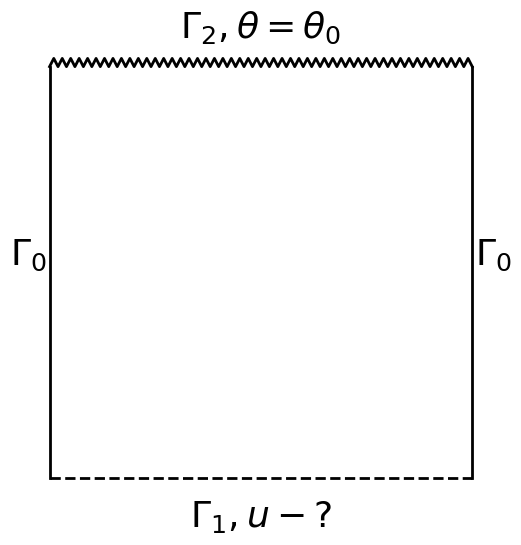
\includegraphics[width=1\linewidth]{omega_1}}
%        \caption*{$\Gamma \coloneqq \partial \Omega =\overline{\Gamma}_0 \cup \overline{\Gamma}_1 \cup \overline{\Gamma}_2$}
    \end{wrapfigure}
    \begin{gather}
        \label{eq:2_1:initial}
        - a \Delta \theta + b \kappa_a(\theta ^ 3 | \theta | - \varphi) = 0, \\
        - \alpha \Delta \varphi + \kappa_a (\varphi - \theta ^3 | \theta |) = 0,
    \end{gather}
    \begin{equation}
        \label{eq:2_1:initial-boundary}
        \begin{aligned}
            \Gamma &: \; a \partial_n \theta + \beta (\theta - \theta _b) = 0, \\
            \Gamma_0 \cup \Gamma_2 &: \; \alpha \partial_n \varphi
            + \gamma(\varphi - \theta_b ^4 ) = 0, \\
            \Gamma_1 &: \; \alpha \partial_n \varphi + u(\varphi - \theta_b ^4 ) = 0. \\
        \end{aligned}
    \end{equation}
    $\Gamma_0, \Gamma_1, \Gamma_2$ не имеют пересечений.

    Функции $\gamma, \theta_b, \beta$ известны.
    \textit{Неизвестная функция $u$ характеризует отражающие свойства участка границы $\Gamma_1$}.
    Предполагается, что $0 < u_1 \leq u \leq u_2$.

    \textbf{Обратная задача} заключается в отыскании тройки $\theta, \varphi, u$
    по дополнительному условию $\theta|_{\Gamma_2} = \theta_0$.

    \textbf{Экстремальная задача} заключается в минимизации функционала
    \begin{equation}
        \label{eq:2_1:quality}
        J(\theta) = \frac{1}{2} \int_{\Gamma_2} (\theta - \theta_0)^2 d\Gamma
    \end{equation}
    на решениях краевой задачи~\eqref{eq:2_1:initial}--\eqref{eq:2_1:initial-boundary}.
\end{frame}
\note{
    \begin{itemize}
        \item Первая из рассматриваемых задач представляется двумя уравнениями ...
        \item Пару $\theta, \varphi$ - будем называть состоянием системы.
        \item Дополняется граничными условиями ...
        \item Если же параметр отражательной способности неизвестен на части границы,но ...
        \item Неизвестные параметры среды мы будем называть функцией управления $u$.
        В данном случае, неизвестен параметр $\gamma$ на нижней границе.
        \item Краевая задача, где все параметры среды известны хорошо изучена, (АЮ 2015)
        \item Об обратной задаче нет данных - формулируем задачу опт. управления.
        \item Квазирешение и его существование.
    \end{itemize}
}


\begin{frame}
    \frametitle{Нахождение квазирешения обратной задачи}
    \begin{gather}
        A_1 \theta + b \kappa_a (| \theta | \theta^3 - \varphi) =
        f, A_2 \varphi + \kappa_a (\varphi - |\theta|\theta^3) + F(\varphi, u) = g.
        \label{eq:2_1:weakOperational}\\
        J(\theta) = \frac{1}{2} \int_{\Gamma_2} (\theta - \theta_0)^2 d\Gamma,
        \label{eq:2_1:qualityOperational}\\
        A_1 p_1 + 4 |\hat{\theta}|^3 \kappa_a(b p_1 - p_2) = f_c,
        \;\; (f_c,v) = - \int_{\Gamma_2} (\hat{\theta} - \theta_0) v d\Gamma,
        \label{eq:2_1:theorem_2_eq1}\\
        A_2 p_2 + \kappa_a (p_2-b p_1) = g_c(p_2, \hat{u}),
        \;(g_c(p_2, \hat{u}), v) = -\int_{\Gamma_1} \hat{u} p_2 v d\Gamma,
        \label{eq:2_1:theorem_2_eq2}\\
        \int_{\Gamma_1} p_2 (\hat{\varphi} - \theta_b^4)(u-w) d\Gamma
        \leq 0 \quad \forall w \in U_{ad}. \label{eq:2_1:theorem_2_eq3}
    \end{gather}
    \textbf{Алгоритм градиентного спуска с проекцией}
    \begin{enumerate}
        \item Выбор шага $\lambda$, числа итераций $N$, управления $u_0 \in U_{ad}$
        -- пространство допустимых управлений.
        \item для $k \leftarrow 0,1,2, \ldots, N$ выполнить:
        \begin{itemize}
            \item Для $u_{k}$, вычислить $y_k = \{\theta_k, \varphi_k\}$ из~\eqref{eq:2_1:weakOperational}.
            \item Вычислить значение $J(\theta_k)$ из уравнения~\eqref{eq:2_1:quality}.
            \item Рассчитать $p_k=\{p_{1k},p_{2k}\}$
            из~\eqref{eq:2_1:theorem_2_eq1}--\eqref{eq:2_1:theorem_2_eq2},
            \item Пересчитать управление
            $u_{k+1} = P_{ad}\left[ u_k - \lambda (\varphi_k - \theta_b^4)p_{2k} \right]$.
        \end{itemize}
    \end{enumerate}
\end{frame}
\note{
    Предложенный в работе алгоритм поиска квазирешения обратной задачи основан
    на выведенных условиях оптимальности
    (доказано, что квазирешение должно
    удовлетворять~\eqref{eq:2_1:weakOperational}--\eqref{eq:2_1:theorem_2_eq2}),
    куда входят сопряженные функции для температуры $p_1$ и излучения $p_2$,
    а также связь между сопряженным состоянием и искомым граничным управлением.
    Для компактной записи краевых задач, используется современная операторная форма.
    Система~\eqref{eq:2_1:weakOperational} является операторной записью краевой задачи,
    где $A_{1,2}$ описывают диффузионные члены модели, остальные моделируют граничные условия.
    Уравнения~\eqref{eq:2_1:theorem_2_eq1}--\eqref{eq:2_1:theorem_2_eq2}
    это сопряженная система,
    а вариационное неравенство~\eqref{eq:2_1:theorem_2_eq3}
    устанавливает связь с оптимальным управлением.

    Приведём алгоритм градиентного спуска с проекцией.
    Обратим внимание, что оператор проекции нужен
    из-за начальных ограничений на функцию управления
    (вызванных физичностью параметра, например).

    Отметим, что в силу невыпуклости экстремальной задачи градиентные алгоритмы не обладают
    свойством глобальной сходимости, что служит основой для их критики, зачастую заслуженной.

    Однако свойства диффузионных моделей сложного теплообмена представленные в диссертации
    и правильный выбор шага градиентного метода обеспечивают сходимость для
    рассматриваемых задач.
    Следующие примеры этот факт демонстрируют.
}

\begin{frame}
    \textbf{Численные эксперименты:}

    \begin{wrapfigure}{r}{0.3\textwidth}
        \centering{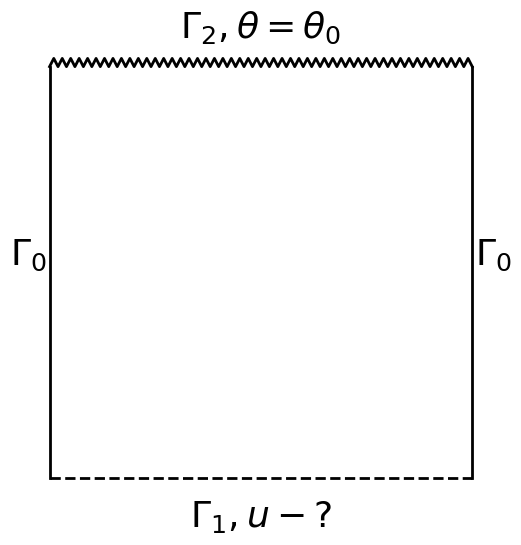
\includegraphics[width=1\linewidth]{omega_1}}
%        \caption*{$\Gamma \coloneqq \partial \Omega =\overline{\Gamma}_0 \cup \overline{\Gamma}_1 \cup \overline{\Gamma}_2$}
    \end{wrapfigure}
    Положим $\Omega = \{(x,y), 0 \leq x,y \leq 1\}$, $l = 1$ см.
    Граница $\partial\Omega$:
    \[
        \begin{aligned}
            \Gamma_0 & = \{x=\{0,1\}, y \in [0,1]\} \\
            \Gamma_1 & = \{x\in [0,1], y=0\}
            - \text{участок с неизвестными отр. свойствами}, \\
            \Gamma_2 & = \{x \in [0,1], y=1\} - \text{участок наблюдения}.
        \end{aligned}
    \]
    Будем также далее считать, что $a = 0.006[\text{см}^2/\text{c}]$,
    $b=0.025[\text{см}/\text{с}]$, $\beta = 0.00005[\text{см}/\text{с}]$,
    $\kappa=1[\text{см}^{-1}]$, $\kappa_s = 0$, $A = 0$, $\gamma = 0.3$.
    Температуру на границе $\Omega$ положим равной $\theta_b = (x^2+y^2)/3$.

    При указанных параметрах для первого эксперимента выберем следующее тестовое
    значение функции $u$:
    \begin{equation*}
        u(x)=
        \begin{cases}
            0.01, & \text{если } x \le 0.5, \\
            0.5, & \text{если } x > 0.5,
        \end{cases}
    \end{equation*}
    и для второго эксперимента:
    $u(x)=0.49x+0.01$.
\end{frame}
\note{
    Положим параметры среды, соответствующие стеклу и зададим тестовую функцию управления
    как показано на слайде.
    Пластинка, у которого боковые стороны "обычные", верхняя грань - участок наблюдения,
    нижняя грань - участок под "контролем".
}


\begin{frame}
    \textbf{Результаты моделирования:}

    \centering
    \includegraphics[width=0.42\linewidth]{dvmg368/1}
    \includegraphics[width=0.42\linewidth]{dvmg368/2}
    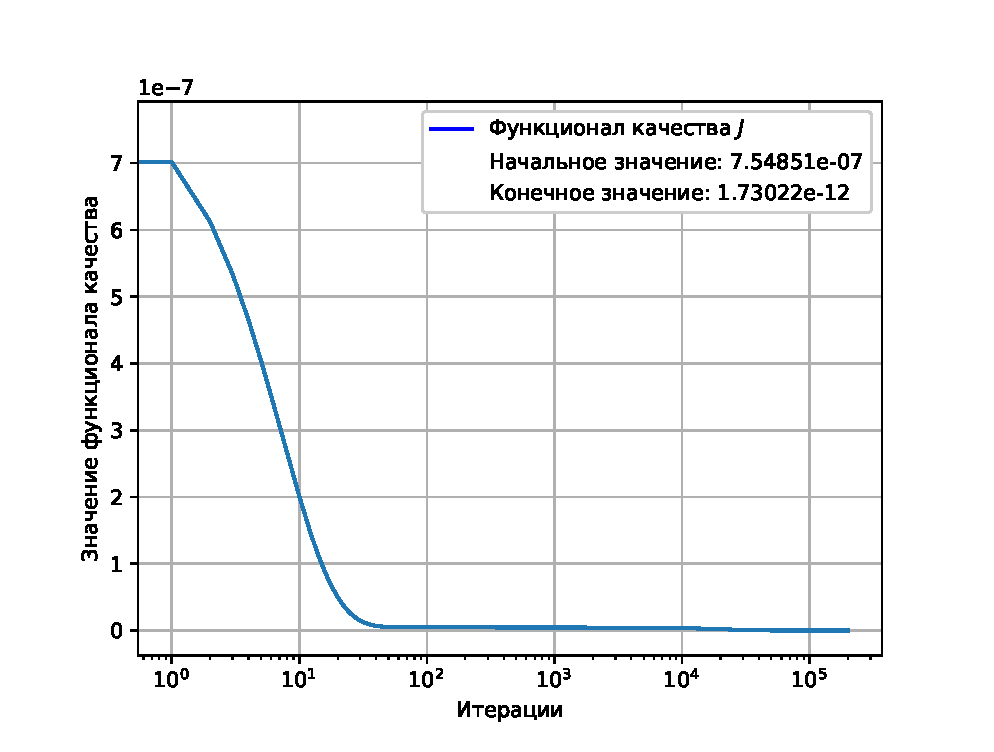
\includegraphics[width=0.42\linewidth]{dvmg368/3}
    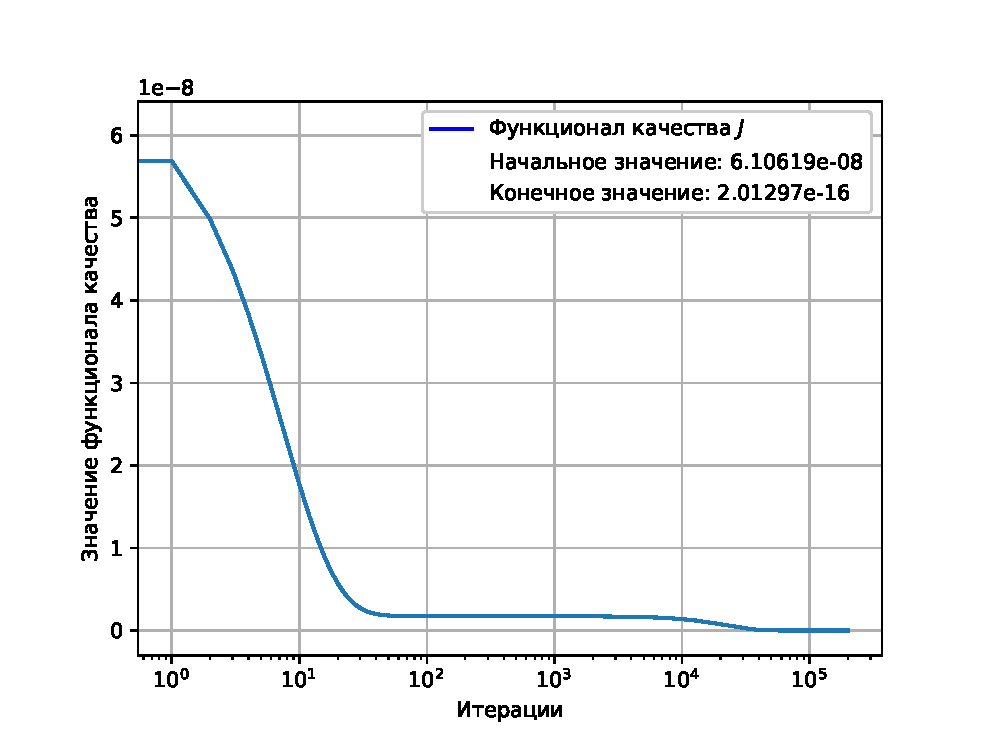
\includegraphics[width=0.42\linewidth]{dvmg368/4}
\end{frame}
\note{
    Интересный эффект "среднего значения". Большое количество итераций.
    Обратить внимание на функционал качества.
    Для получения представленных результатов, использовался разработанный мной комплекс программ,
    включающий решение прямой задачи, сопряженной системы и алгоритм градиентного спуска.
}

\subsection{Обратная задача с условиями типа Коши}\label{subsec:rev_koshi}
\begin{frame}
    \frametitle{Задача без краевых условий для интенсивности излучения}
    \textbf{Краевая задача:}
    \begin{equation}
        \label{eq:2_2:eq1}
        - a \Delta \theta + b \kappa_a(\theta ^ 3 | \theta | - \varphi) = 0,  \quad
        - \alpha \Delta \varphi + \kappa_a (\varphi - \theta ^3 | \theta |) = 0,
    \end{equation}
    На $\Gamma$ известно температурное поле и тепловой поток:
    \begin{equation}
        \label{eq:2_2:bc2} \theta = \theta_b, \quad \partial_n\theta = q_b.
    \end{equation}
    Заменяем на <<искусственные>> краевые условия
    \begin{equation}
        \label{eq:2_2:bc3}
        a(\partial_n\theta+\theta) = r,\;\;
        \alpha(\partial_n\varphi+\varphi) = u \text{ на }\Gamma.
    \end{equation}
    Функция $r(x),\, x\in\Gamma$ является заданной, функция $u(x),\, x\in\Gamma$
    описывающая излучающие свойства участка границы, неизвестна.
    Получаем \textbf{обратную задачу}.

    \textbf{Задача оптимального управления} заключается в отыскании тройки
    $\{\theta_\lambda,\varphi_\lambda,u_\lambda\}$ такой, что
    \begin{equation}
        \label{eq:2_2:cost}
        J_\lambda(\theta, u) = \frac{1}{2}\int\limits_\Gamma (\theta - \theta_b)^2 d\Gamma
        + \frac{\lambda}{2}\int\limits_\Gamma u^2 d\Gamma \rightarrow\inf
    \end{equation}
    на решениях краевой задачи, функция $u(x) x \in \Gamma$ играет роль управления.

    \begin{itemize}
        \item $(j) \;\; a,b,\alpha,\kappa_a, \lambda ={\textrm Const}> 0,$
        \item $(jj) \;\, \theta_b, \,q_b \in U,\;\; r=a(\theta_b+q_b)$.
    \end{itemize}
    \begin{theorem}[2.5]
        \label{th:2_2:3}
        Пусть выполняются условия $(j),(jj)$ и существует решение
        задачи~\eqref{eq:2_2:eq1}--\eqref{eq:2_2:bc2}.
        Если $\{\theta_\lambda,\varphi_\lambda,u_\lambda\}$ -- решение
        задачи оптимального управления для $\lambda>0$, то существует последовательность $\lambda\to +0$
        такая, что
        $\theta_\lambda\rightarrow\theta_*, \;\; \varphi_\lambda\rightarrow\varphi_*
        \text{ слабо в }V,\text{ сильно в }H$,
        где $\theta_*,\varphi_*$ -- решение задачи~\eqref{eq:2_2:eq1}--\eqref{eq:2_2:bc2}.
    \end{theorem}
\end{frame}
\note{
    23. Не задано $\varphi$!
    В основе разработанного алгоритма решения лежит анализ экстремальной задачи.

    Строго обосновано существование решения экстр задачи.
    Кроме того, и это принципиально важно, показана сходимость решений экстремальных задач
    к решению задачи~\eqref{eq:2_2:eq1}--\eqref{eq:2_2:eq2}
    без краевых условий для интенс излучения при $\lambda$ стремящемся к 0.
}
\begin{frame}
    \textbf{Разрешимость задачи оптимального управления и условия оптимальности}

    \begin{theorem}[2.3]
        \label{th:2_2:1}
        Пусть выполняются условия $(j), (jj)$.
        Тогда существует решение задачи $CP$.
    \end{theorem}
    \begin{theorem}[2.4]
        \label{th:2_2:2}
        Пусть выполняются условия $(j),(jj)$.
        Если $\{\hat{\theta}, \hat{\varphi}, \hat{u}\}$ -- решение задачи оптимального управления,
        то существует единственная пара $\{p_1, p_2 \} \in V\times V$ такая, что
        \begin{equation}
            \label{eq:2_2:as}
            aAp_1 +4|\hat{\theta}|^3 \kappa_a(bp_1 - p_2) = B(\theta_b - \hat{\theta}), \;\;
            \alpha A p_2 + \kappa_a (p_2 - b p_1)=0
        \end{equation}
        и при этом $\lambda\hat{u} = p_2$.
    \end{theorem}


    \textbf{Алгоритм решения задачи без краевых условий для интенсивности излучения}

    1.\ Выбираем значение градиентного шага $\varepsilon$,

    2.\ Выбираем количество итераций $N$,

    3.\ Выбираем начальное приближение для управления $u_{0} \in U$,

    4.\ для $k \leftarrow 0,1,2, \ldots, N$ выполнить:

    \hspace{1cm} a.\ Для заданного $u_{k}$, вычислить состояние
    $y_{k}=\left\{\theta_{k}, \varphi_{k}\right\}$, решение
    задачи~\eqref{eq:2_2:eq1}--\eqref{eq:2_2:bc1}.

    \hspace{1cm} b.\ Вычислить значение функционала качества
    $J_{\lambda}\left(\theta_{k}, u_{k}\right)$.

    \hspace{1cm} c.\ Из уравнений~\eqref{eq:2_2:as}, вычислить сопряженное
    состояние $p_{k}=\left\{p_{1k}, p_{2k}\right\}$,
    где $\widehat{\theta} \coloneqq \theta_{k}, \widehat{u} \coloneqq u_{k}$.

    \hspace{1cm} d.\ Пересчитать управление
    $u_{k+1}=u_{k}-\varepsilon\left(\lambda u_{k}-p_{2}\right)$.


    Значение параметра $\varepsilon$ выбирается эмпирически.
    Количество итераций $N$ выбирается достаточным для выполнения условия
    $J_\lambda(\theta_k, u_k) - J_\lambda(\theta_{k+1}, u_{k+1}) < \delta$, где $\delta>0$
    определяет точность расчетов.
\end{frame}
\note{
    25. Условия оптимальности лежат в основе численного метода
}

\begin{frame}
    \textbf{Пример 1.}
    Приведем примеры расчетов для куба $\Omega = {(x, y, z), 0 \leq x,y,z \leq l}$.

    Будем считать, что $l=1~\text{см}$, $a = 0.006[\text{см}^2/\text{c}]$,
    $b=0.025[\text{см}/\text{с}]$, $\kappa_a=1[\text{см}^{-1}]$, $\alpha = 0.(3)[\text{см}]$.
    Параметр регуляризации $\lambda=10^{-12}$.

    Определим $r$ и $u$ в~\eqref{eq:2_2:bc3} как $r = 0.7, \quad u = \hat u = 0.5$.
    Для обозначенных параметров рассчитаем функции $\theta$, $\varphi$ из решения граничной задачи
    и положим $\theta_b = \theta|_\Gamma$.
    Нормальная производная $\partial_n \theta = q_b = r / a - \theta_b$.

    Применяя алгоритм градиентного спуска найдем решение задачи оптимального управления.
    \begin{figure}[h!t]
        \begin{minipage}[b][][b]{0.49\linewidth}
            \centering
            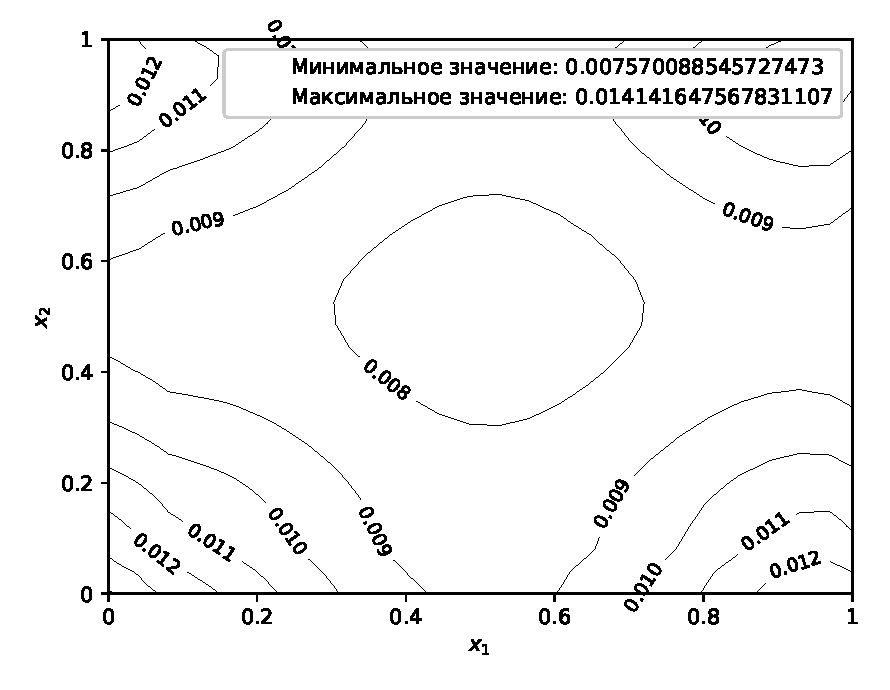
\includegraphics[width=1\linewidth]{jvm-2020/exp1/theta_n_diff_iso}
            \\ а) $|\partial_n\theta_\lambda-q_b|/|q_b|$
        \end{minipage}
        \hfill
        \begin{minipage}[b][][b]{0.49\linewidth}
            \centering
            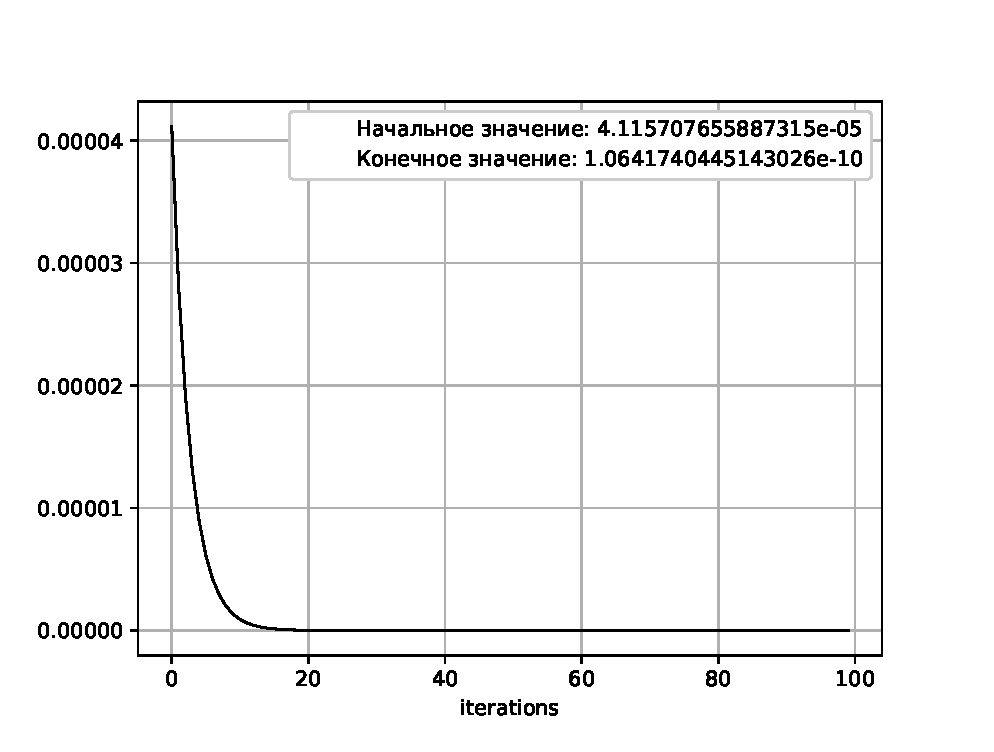
\includegraphics[width=1\linewidth]{jvm-2020/exp1/quality}
            \\ б) Значение функционала качества
        \end{minipage}
        \label{fig:4_4:0}
    \end{figure}
\end{frame}
\note{
    Обратите внимание на малость функционала качества.
    Сравним с тем, что получилось -- довольно близко, но не идеально.
    Уменьшение параметра регуляризации повышает точность решения,
    но и увеличивает вычислительные затраты.
}

\begin{frame}
    \textbf{Пример 2.}


    Зададим функции $\theta_{b}, q_{b}$ в краевом условии~\eqref{eq:2_2:bc2}
    следующим образом:
    \[
        \theta_{b}=0.1 z+0.3, \quad q_{b}=
        \begin{cases}
            0.11, & \text { если } z=1, \\
            0, & \text { если } 0<z<1, \\
            -0.15, & \text { если } z=0.
        \end{cases}
    \]

    В данном примере оптимальное управление $u$ в качестве тестового не задается.
    Начальное значение функционала качества $J_\lambda$ составляет $7.20 \cdot 10^{-6}$.
    Финальное значение $2.86 \cdot 10^{-10}$.

    \begin{figure}[h!t]
        \begin{minipage}[b][][b]{0.49\linewidth}
            \centering
            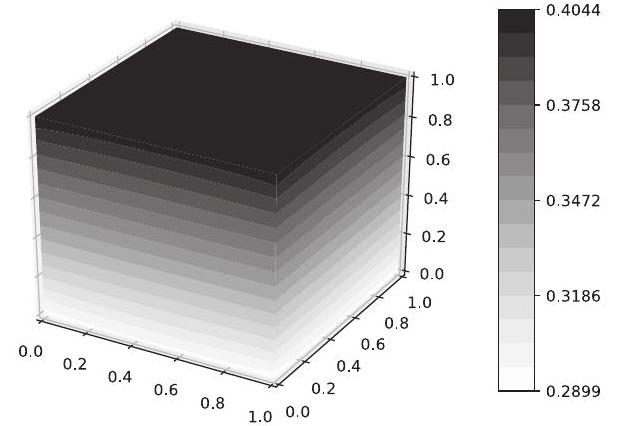
\includegraphics[width=0.9\linewidth]{jvm-2020/dvmg/3b}
            \\ а) Полученное температурное поле $\theta_\lambda$
        \end{minipage}
        \hfill
        \begin{minipage}[b][][b]{0.49\linewidth}
            \centering
            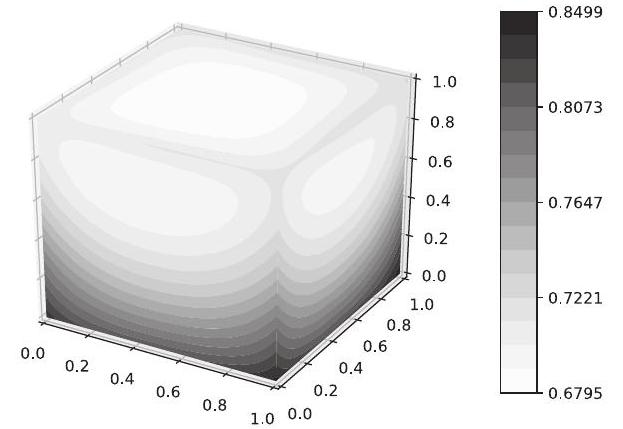
\includegraphics[width=1\linewidth]{jvm-2020/dvmg/2a}
            \\ б) Полученное поле излучения $\varphi_\lambda$
        \end{minipage}
        \label{fig:4_4:3}
    \end{figure}

\end{frame}
\note{
    "Честный" эксперимент - используем то, что полагается в исходной задаче.
    Функционал качества (его динамика) позволяет предположить аналогичный порядок
    близости (с предыдущим примером)
    точного и аппроксимированного решений.
    Обратите внимание на линейность $\theta_b$ по оси $z$.
}


\subsection{Квазистационарная задача с данными Коши}\label{subsec:qst_koshi}
\begin{frame}
    \frametitle{Квазистационарная модель с данными Коши}
    \textbf{Начально-краевая задача:}
    \begin{equation}
        \label{eq:2_3:1}
        \begin{split}
            & \frac{\partial \theta}{\partial t} - a \Delta \theta
            + b \kappa_{a} \left(|\theta| \theta^{3}-\varphi\right) = 0,\\
            & - \alpha \Delta \varphi
            + \kappa_{a} \left(\varphi-|\theta| \theta^{3}\right) = 0,
            \quad x \in \Omega, \quad 0 < t < T;
        \end{split}
    \end{equation}
    \begin{align}
        a \left(\partial_{n} \theta+\theta\right)=r,
        & \quad \alpha\left(\partial_{n} \varphi
        + \varphi\right) = u \text { на } \Gamma;  \label{eq:2_3:2}\\
        & \left.\theta\right|_{t=0} = \theta_{0}. \label{eq:2_3:3}
    \end{align}


    \textbf{Экстремальная задача} состоит в том, чтобы найти тройку
    $\left\{\theta_{\lambda}, \varphi_{\lambda}, u_{\lambda}\right\}$ такую, что
    \begin{equation}
        \label{eq:2_3:4}
        J_{\lambda}(\theta, u)=\frac{1}{2} \int_{0}^{T}
        \int_{\Gamma}\left(\theta-\theta_{b}\right)^{2} d \Gamma d t+\frac{\lambda}{2}
        \int_{0}^{T} \int_{\Gamma} u^{2} d \Gamma d t \rightarrow \inf
    \end{equation}
    на решениях задачи~\eqref{eq:2_3:1}--\eqref{eq:2_3:3}.
    \begin{itemize}
        \item $(k)\; a, b, \alpha, \kappa_{a}, \lambda=$ Const $>0$,
        \item $(kk)\; \theta_{b}, q_{b} \in U, r=a\left(\theta_{b}+q_{b}\right)
        \in L^{5}(\Sigma), \; \theta_{0} \in L^{5}(\Omega)$.
    \end{itemize}


    \begin{theorem}[2.8]
        \label{th:2_3:3}
        Пусть выполняются условия $(k), (kk)$ и существует решение
        $\theta, \varphi \in$ $L^{2}\left(0, T ; H^{2}(\Omega) \right)$
        задачи~\eqref{eq:2_3:1}--\eqref{eq:2_3:3}.
        Если $\left\{\theta_{\lambda}, \varphi_{\lambda}, u_{\lambda}\right\}$
        — решение задачи $OC$ при $\lambda>0$, то при $\lambda\rightarrow+0$
        \[
            \begin{gathered}
                \theta_{\lambda} \rightarrow \theta \text { слабо в } L^{2}(0, T ; V),
                \text { сильно в } L^{2}(Q), \\
                \varphi_{\lambda} \rightarrow \varphi \text { слабо в } L^{2}(0, T ; V).
            \end{gathered}
        \]
    \end{theorem}
\end{frame}
\note{
    27. Аналог стационарной задачи с небольшими сдвигами по времени.
    Для оптимизационного метода решения задачи требуются результаты анализа кв.стц. модели из гл. 1!
    параметр u неизвестен.
}

\begin{frame}
    Область $\Omega \times(-L, L)$,
    где $\Omega=$ $\left\{x=\left(x_{1}, x_{2}\right): 0<x_{1,2}<d\right\}$.


    Определим параметры:
    $d=1(\text{м})$, $a=0.9210^{-4}(\text{м}^{2} / \text{с})$,
    $b=0.19(\text{м} / \text{с})$, $\alpha=0.0333(\text{м})$,
    $\kappa_{a}=1\left(\text{м}^{-1}\right)$, $T = 1(\text{c})$.
    \begin{figure}[h!t]
        \begin{minipage}[b][][b]{0.49\linewidth}
            \centering
            \includegraphics[width=1\linewidth]{paper03/1} \\ а) Поле температуры,
            полученное в статье *
        \end{minipage}
        \hfill
        \begin{minipage}[b][][b]{0.49\linewidth}
            \centering
            \includegraphics[width=1\linewidth]{paper03/2} \\
            б) Поле температуры, полученное предложенным алгоритмом
        \end{minipage}
        \label{fig:4_3:1}
    \end{figure}
    \tiny{* A. Y. Chebotarev, A. E. Kovtanyuk и N. D. Botkin. — \textit{«Problem of
    radiation heat exchange with boundary conditions of the Cauchy type»}. —
    Communications in Nonlinear Science and Numerical Simulation 75 (2019),
        с. 262—269.}
\end{frame}
\note{

    52. Приведены изображения сравнения полученных результатов в рамках работы
    над диссертацией и коллег из Мюнхена (финальный момент времени)
    Параметры среды соответствуют воздуху при нормальном атмосферном давлении и температуре 400C.


    N.Botkin для расчетов использовал, разработанную в TUM программу, использующую
    эрмитов прямоугольный (конформный) элемент Богнера-Фокса-Шмидта и сведение задачи к нестационарной.
    Не ясно, что же такое случилось с пространством решений,
    что потребовались столь экзотические конечные элементы.

    Фактически ему пришлось решать краевую задачу для нелинейного уравнения 4 порядка.
    Предложенный в работе оптимизационный алгоритм является более простым и дает фактически те же результаты.
    Использовались конечные элементы Галёркина (Лагранжа-1).

}

\subsection{Стационарная задача с условиями Коши на части границы}\label{subsec:st-koshi}
\begin{frame}
    \frametitle{Стац.\ задача с условиями Коши для температуры на части границы}
    \begin{wrapfigure}{r}{0.4\textwidth}
        \centering{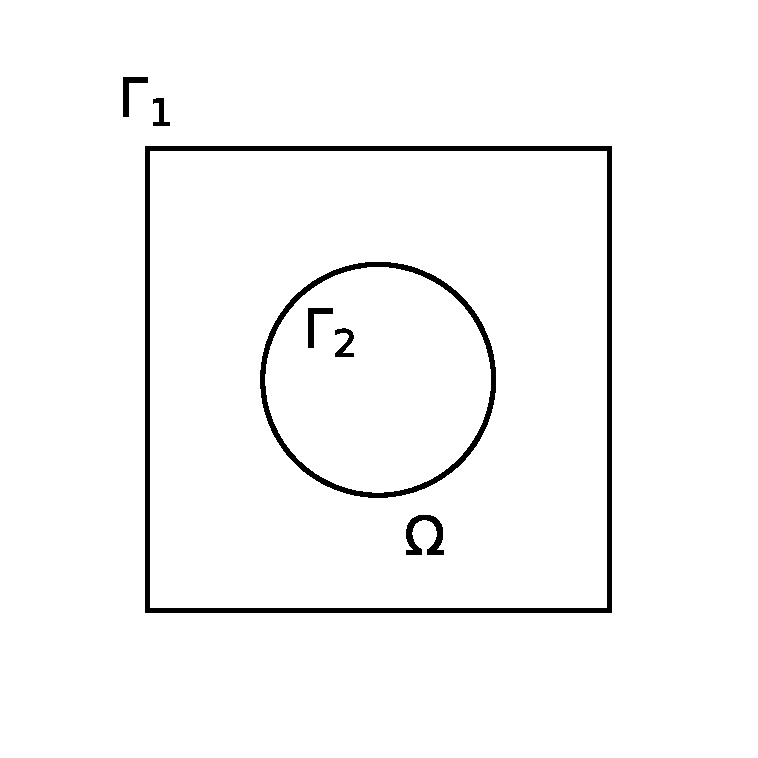
\includegraphics[width=1\linewidth]{omega-circle}}
%        \caption*{$\Gamma \coloneqq \partial \Omega =\overline{\Gamma}_0 \cup \overline{\Gamma}_1 \cup \overline{\Gamma}_2$}
    \end{wrapfigure}
    Рассмотрим область $\Omega$ с границей $\Gamma=\partial\Omega$.
    \begin{gather}
        \label{eq:2_4:eq1}
        - a\Delta\theta + b\kappa_a(\theta^4 - \varphi) = 0,   \\
        -\alpha \Delta \varphi + \kappa_a(\varphi- \theta^4) = 0.
    \end{gather}
    $\Gamma \coloneqq \partial \Omega =\overline{\Gamma}_1 \cup \overline{\Gamma}_2$
    так, что $\Gamma_1 \cap \Gamma_2 =  \emptyset$.
    На всей границе $\Gamma$ задается тепловой поток $q_b$,
    \begin{equation}
        \label{eq:2_4:bc1}
        a\partial_n\theta = q_b, \quad x\in \Gamma.
    \end{equation}
    Для задания краевого условия для интенсивности излучения требуется знать функцию $\gamma$.
    В случае, если эта функция неизвестна на части границы $\Gamma_2$,
    краевое условие для интенсивности излучения на $\Gamma_2$ не ставится, а в качестве условия
    переопределения на $\Gamma_1$, в дополнение к условию на
    $\varphi$, задается температурное поле $\theta_b$,
    \begin{equation}
        \label{eq:2_4:bc2}
        \alpha\partial_n\varphi + \gamma (\varphi - \theta_{out} ^4 ) = 0,\;
        \theta=\theta_b\quad \text{ на } \Gamma_1.
    \end{equation}.

\end{frame}
\note{
    30. Рассмотрим случай если на всей границе известен поток, а параметр из гранич. условия
    для $\varphi$ неизвестен. Мы дополняем "доступный" участок информацией о температуре: $theta_b$.
    Если данные Коши заданы на части границы задача является ещё более сложной.
    Для точной постановки нет результатов по её корректности.
    Однако предлагаемый далее оптимизационный метод полностью теоретически обоснован и
    лежит в основе соответствующего программного комплекса для численного решения.
}
% % чтобы не пугать никого, математическая эквилибристика на слайде спрятана под ковёр.
%\begin{frame}
%    \textbf{Постановка задачи управления}
%
%
%    Введем новую неизвестную функцию
%    $\psi= a\theta + \alpha b \varphi$.
%
%    \textbf{Краевая задача}:
%    \begin{equation}
%        \label{eq:2_4:eq2}
%        - a \Delta \theta + g (\theta) = \frac{\kappa_a}{\alpha}\psi, \quad
%        \Delta \psi = 0, \; x \in \Omega,
%    \end{equation}
%    \begin{equation}
%        \label{eq:2_4:bc3}
%        a \partial_n \theta = q_b \; \text{ на }\Gamma, \;\;
%        \alpha \partial_n \psi + \gamma \psi  =  r,\;\;
%        \theta = \theta_b  \text{ на }\Gamma_1.
%    \end{equation}
%    Здесь $g(\theta) = b \kappa_a|\theta|\theta^3 + \frac{a\kappa_a}{\alpha}\theta$, $r=\alpha b \gamma \theta_{out}^4+ \alpha q_b + a \gamma \theta_b$.
%
%
%    Задача \textbf{оптимального управления}, аппроксимирующая краевую задачу,
%    заключается в отыскании тройки $\{\theta_\lambda,\psi_\lambda,u_\lambda\}$ такой, что
%    \begin{gather}
%        \label{eq:2_4:cost}
%        J_\lambda(\theta, u) =
%        \frac{1}{2} \int \limits_{\Gamma_1} (\theta - \theta_b)^2 d \Gamma
%        + \frac{\lambda}{2}\int\limits_{\Gamma_2} u^2 d\Gamma \rightarrow \inf, \\
%        - a \Delta \theta + g (\theta) = \frac{\kappa}{\alpha}\psi, \quad
%        \Delta \psi = 0, \; x \in \Omega, \\
%        a \partial_n \theta + s \theta = q_b + s \theta_b,
%        \; \alpha \partial_n \psi + \gamma \psi = r
%        \text{ на } \Gamma_1,\\
%        a \partial_n \theta = q_b, \;
%        \alpha \partial_n \psi = u \text{ на } \Gamma_2.
%    \end{gather}
%    $\lambda, s > 0$ -- регуляризирующие параметры.
%
%
%    \begin{itemize}
%        \item $(l) \; a,b,\alpha,\kappa_a, \lambda, s ={\textrm Const}> 0.$
%        \item $(ll) \; 0<\gamma_0\leq \gamma \in L^\infty(\Gamma_1), \; \theta_b, r \in L^2(\Gamma_1),\; q_b\in L^2(\Gamma)$.
%    \end{itemize}
%
%    \begin{theorem}[2.9]
%        \label{th:2_4:1}
%        При выполнении условий $(l), (ll)$ существует решение задачи оптимального управления.
%    \end{theorem}
%
%\end{frame}
%\note{
%    31. Используя замену, представленную на слайде, мы заменим исходную задачу, на краевую задачу
%    с функциями $\theta$, $\psi$.
%    Вместо системы двух нелинейных уравнений одно уравнение стало линейным (для $\Psi$)
%    (!!!Где нелинейность в исходной задаче!!!)
%    Два нелинейных заменили на нелинейное и линейное (пси - гармоническая, к тому же).
%    Особо обратим внимание на параметр s, который пришлось добавить в данную постановку из-за
%    того, что реализованный алгоритм не сходился. (Потеря точности решения.?)
%
%    Расчёты выполнены при лямбда равной нулю.
%}

\begin{frame}
    \textbf{Численное моделирование.}


    Рассмотрим двумерный случай:

    Квадрат $S = \{(x, y), 0 \leq x,y,z \leq 1~\text{см.}\}$ с
    круговой полостью $R$ с центром $b_0 =\{0.5, 0.5\}$
    $R = \{r, \| r - b_0 \| \leq 0.15~\text{см.} \}$.

    Рассматриваемая область $\Omega = S \setminus R$.
    $\Gamma \equiv \partial \Omega = \partial C \cup \partial B$, при этом
    $ \Gamma_2 = \partial R, \Gamma_1 = \partial S \setminus \Gamma_2$.
    Граничные данные $q_b$ и $\theta_b$ положим равными
    $
    \theta_b = 0.5, \;
    q_b =
    \begin{cases}
        0.2, & \text{если } x \in \Gamma_1 \\
        -0.2, & \text{если } x \in \Gamma_2.
    \end{cases}
    $
    \begin{figure}[h!t]
        \begin{minipage}[b][][b]{0.49\linewidth}
            \centering
            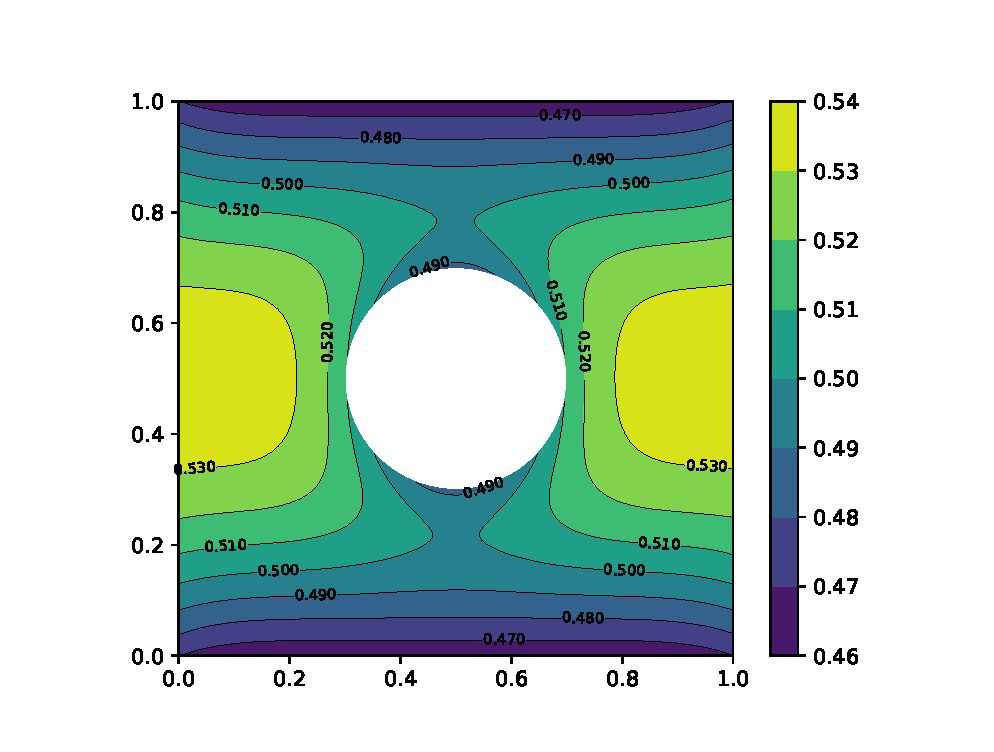
\includegraphics[width=1\linewidth]{theta_endf}
            \\ а) $\theta$
        \end{minipage}
        \hfill
        \begin{minipage}[b][][b]{0.49\linewidth}
            \centering
            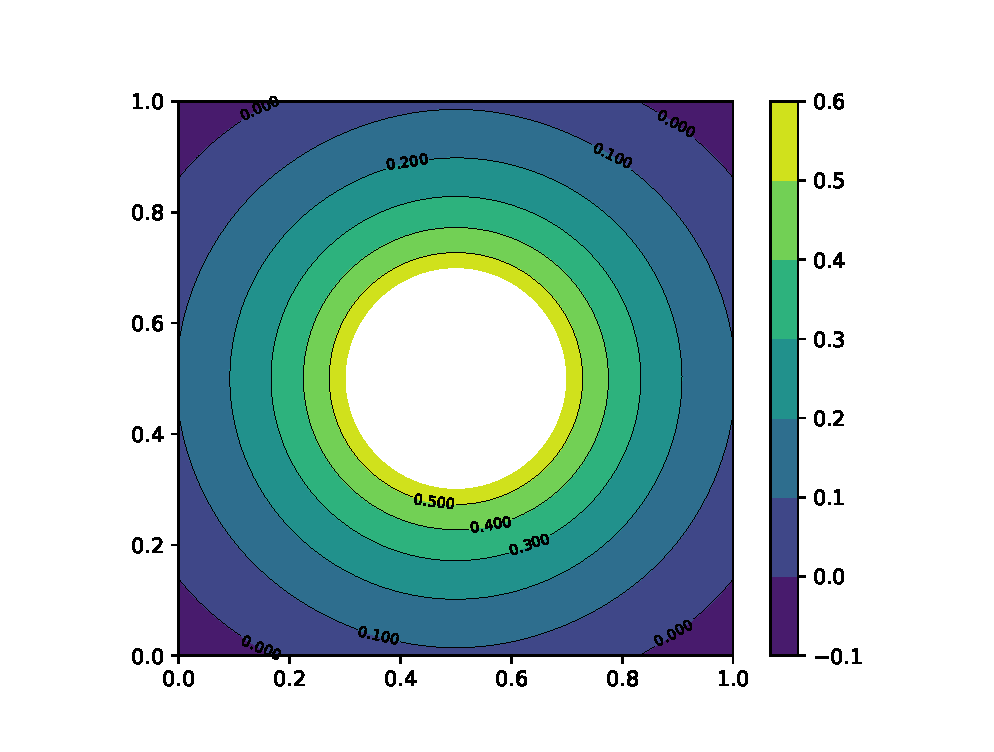
\includegraphics[width=1\linewidth]{phi_endf}
            \\ б) $\varphi$
        \end{minipage}
        \label{fig:4_4:6}
    \end{figure}
    Начальное значение функционала качества $0.045$
    после тридцати итераций становится равным $6.2\cdot10^{-5}$.
\end{frame}
\note{
    63. Квадрат с полостью внутри. (не доступная среда).
}
\begin{frame}
    \frametitle{Исследование устойчивости решений обратных задач с данными Коши}
    Положим $a\partial_n \theta = q_b +\varepsilon \psi$, где $\psi = \psi(x)$, $x \in \Gamma_1$ функция возмущения.

    Полученное решение задачи~\eqref{eq:2_4:eq1},~\eqref{eq:2_4:bc2} обозначим за $\theta^{\varepsilon}$.
    $\theta$ будет соответствовать случаю $\varepsilon = 0$.

    Область $\Omega$ -- квадрат с единичной стороной, $\Gamma_1$ соответствует стороне $y = 1$.

    Положим $\theta_b = (x + y) / 2$ и $q_b = a / 2$, $\varepsilon \in [-0.1, 0.1]$,
    вычислим $L^2$ норму отклонения возмущенного поля.
    \begin{figure}[h!t]
        \begin{minipage}[b][][b]{0.4\linewidth}
            \centering
            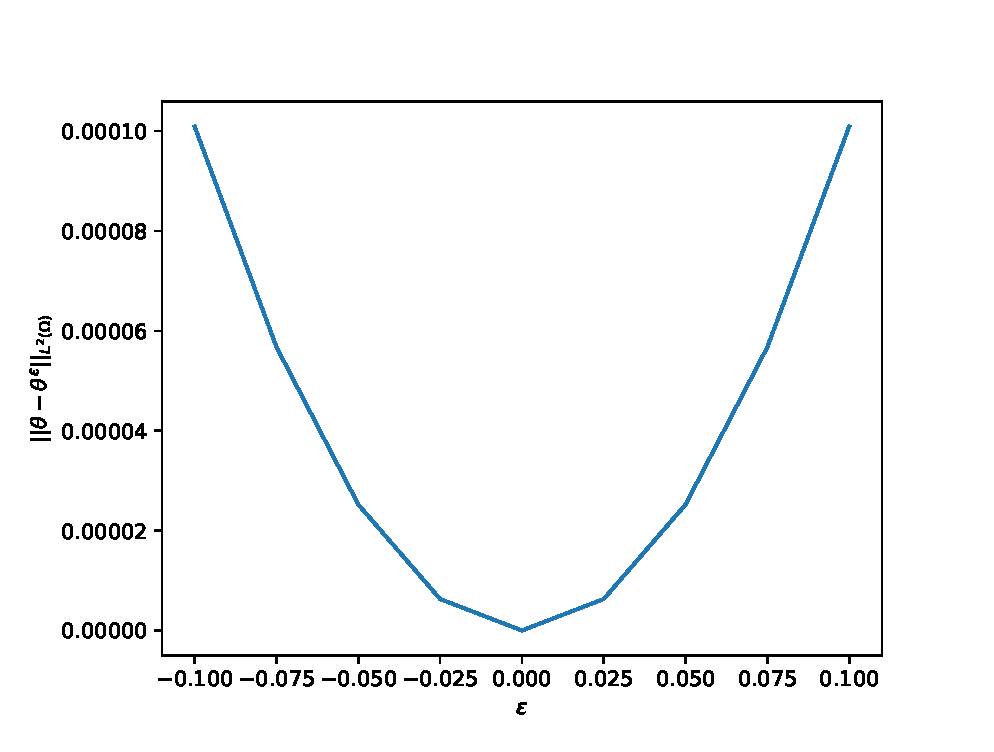
\includegraphics[width=1\linewidth]{additional/2/deps_1}\\ а) $\psi = 1,$
        \end{minipage}
        \hfill
        \begin{minipage}[b][][b]{0.4\linewidth}
            \centering
            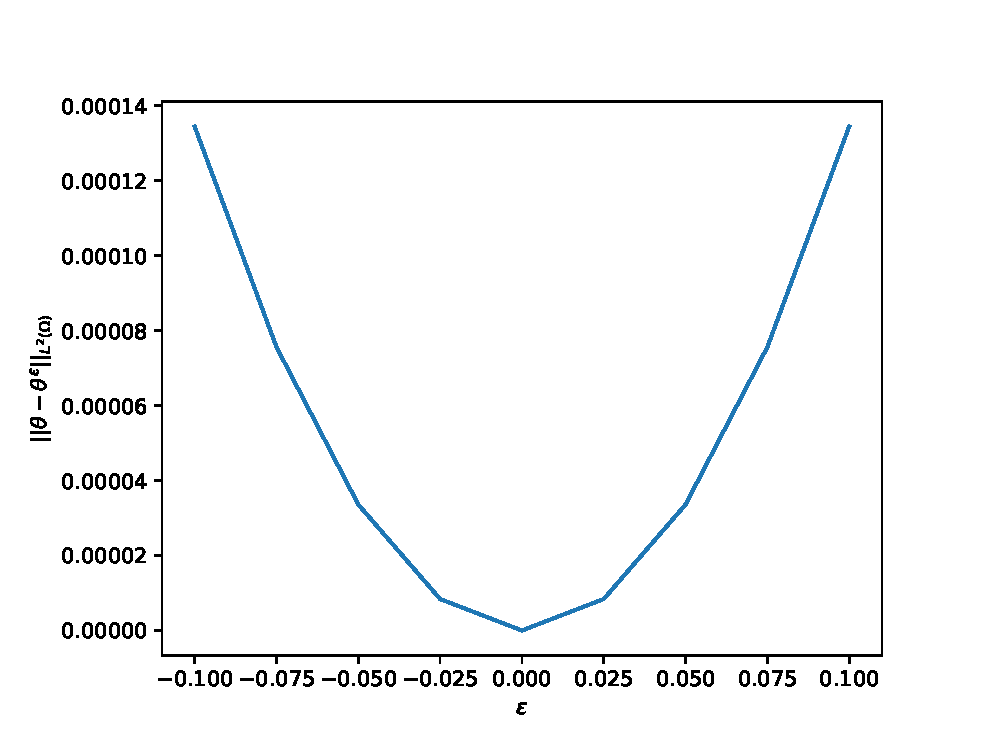
\includegraphics[width=1\linewidth]{additional/2/eps_sin} \\ б) $\psi = \sin (100 * \pi x)$.
        \end{minipage}
        \caption{$||\theta^\varepsilon - \theta||_{L^2(\Omega)}$}
        \label{fig:4_4:vareps}
    \end{figure}
    Численные эксперименты демонстрируют
    устойчивость решения относительно изменений теплового потока.
\end{frame}
\note{
    Также приведем результаты по исследованию устойчивости решений
    обратных задач с данными Коши.
    Для этого переопределим в уравнении~\eqref{eq:2_4:bc3} $a\partial_n \theta = q_b +\varepsilon \psi$,
    где $\psi = \psi(x), x \in \Gamma_1$ некоторая функция, моделирующая возмущение.
    Полученное таким образом решение задачи~\eqref{eq:2_4:eq2},~\eqref{eq:2_4:bc3}
    обозначим за $\theta^{\varepsilon}$.
    Следовательно, $\theta$ будет соответствовать случаю $\varepsilon = 0$.
    Для проведения численного моделирования область $\Omega$ определим
    как квадрат с единичной стороной, где $\Gamma_1$ соответствует стороне $y = 1$.
    Положим $\theta_b = (x + y) / 2$ и $q_b = a / 2$ соответственно.
    Выполним расчеты температурного поля
    для различных малых значений параметра возмущений $\varepsilon$
    из промежутка $[-0.1, 0.1]$ и вычислим $L^2$ норму отклонения возмущенного поля.


    Хорошо известно, что решение задачи с данными
    Коши на границе для одного эллиптического уравнения,
    напр.\ уравнения Лапласа, неустойчиво
    (знаменитый пример Адамара, когда малые изменения
    теплового потока на границе приводят к большим изменениям решения).
    Для рассматриваемой новой модели сложного теплообмена с данными Коши
    теоретический анализ устойчивости это открытая проблема.

    На первом этапе этот вопрос был исследован численно с использованием
    разработанного комплекса программ.

    Полученные численные результаты позволяют высказать гипотезу
    об устойчивости решения этой модели, которую в дальнейшем планируется обосновать аналитически.

}


\section{Задачи оптимального управления для квазилинейных моделей}\label{sec:opt}

\subsection{Задачи оптимального управления с ограничениями на состояние системы и метод штрафа}\label{subsec:opt-phase}
\begin{frame}
    \frametitle{Квазилинейная модель c фазовыми ограничениями}
    \begin{wrapfigure}{r}{0.34\textwidth}
        \centering{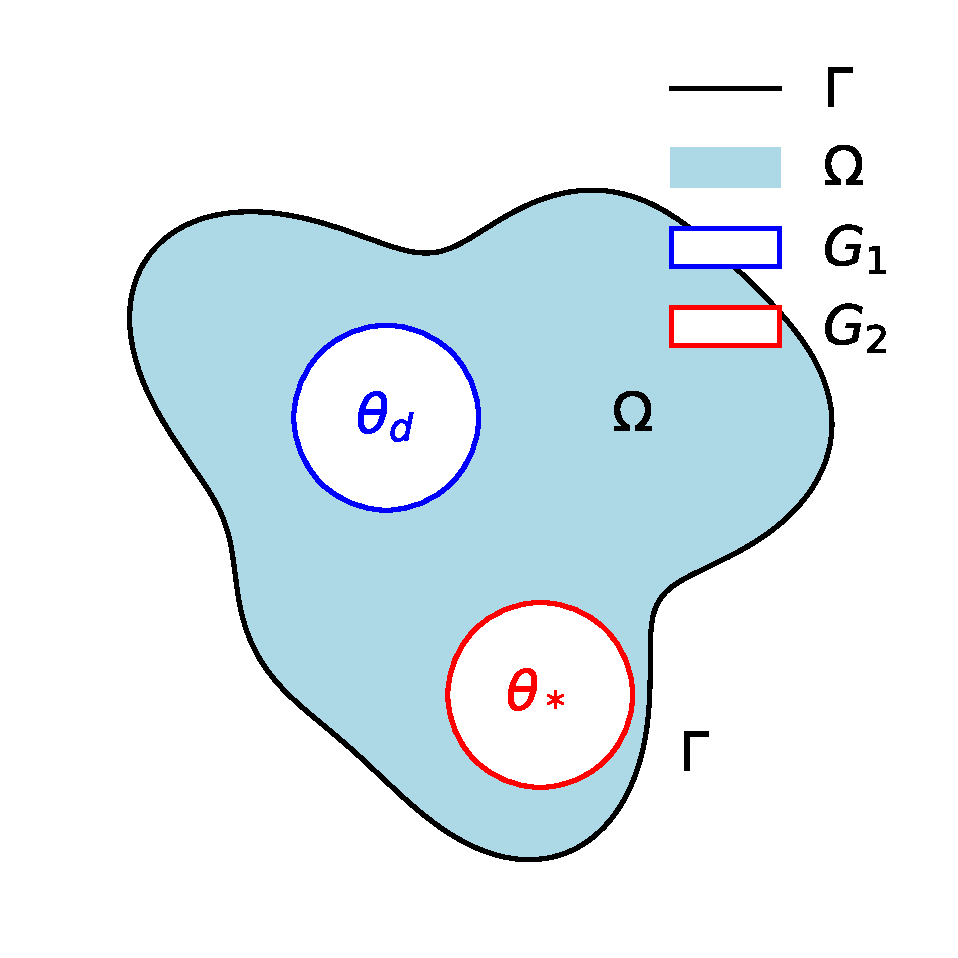
\includegraphics[width=1\linewidth]{omega-g1-g2}}
%        \caption*{$\Gamma \coloneqq \partial \Omega =\overline{\Gamma}_0 \cup \overline{\Gamma}_1 \cup \overline{\Gamma}_2$}
    \end{wrapfigure}

    \textbf{Задача оптимального управления $P$} \\
    заключается в минимизации функционала
    \[ J(\theta)=\int_{0}^{T} \int_{G_{1}}\left(\theta-\theta_{d}\right)^{2} dx dt \rightarrow \inf \]
    на решениях начально-краевой задачи:
    \begin{equation}
        \label{eq:3_2:1}
        \begin{gathered}
            \sigma \partial \theta / \partial t-\operatorname{div}(k(\theta)
            \nabla \theta)-\beta \varphi=u_{1} \chi \\
            -\operatorname{div}(\alpha \nabla \varphi)+\beta \varphi=u_{2}
            \chi, \quad x \in \Omega, \quad t \in(0, T),
        \end{gathered}
    \end{equation}
    \begin{equation}
        \label{eq:3_2:2}
        \theta=\left.0\right|_{\Gamma},
        \quad \alpha \partial_{n} \varphi
        +\left.2^{-1} \varphi\right|_{\Gamma}=0,
        \left.\quad \theta\right|_{t=0}=\theta_{0}.
    \end{equation}
    При этом учитываются ограничения:
    \[ u_{1,2} \geq 0, \quad u_{1}+u_{2} \leq P, \left.\quad \theta\right|_{G_{2}} \leq \theta_{*} \]

    \textbf{Задача со штрафом $P_{\varepsilon}$}.
    $J_{\varepsilon}(\theta) \rightarrow \inf$, где
    \[
        \begin{aligned}
            & J_{\varepsilon}(\theta)=\int_{0}^{T}
            \int_{G_{1}}\left(\theta-\theta_{d}\right)^{2} dx dt
            +\frac{1}{\varepsilon} \int_{0}^{T}
            \int_{G_{2}} F(\theta) d x d t, \\
            & \sigma \theta^{\prime}+A(\theta)=u,
            \quad \theta(0)=\theta_{0}, \quad u \in U_{a d},\\
            &F(\theta)=
            \begin{cases}
                0, & \text { если } \theta \leq \theta_{*} \\
                \left(\theta-\theta_{*}\right)^{2},
                & \text { если } \theta>\theta_{*}.
            \end{cases}
        \end{aligned}
    \]

\end{frame}
\note{
    Дана область, в ней две подобласти. Мы хотим в одной достичь определенного температурного режима,
    в другой хотим не допустить превышения заранее заданного ограничения.
    $P$ – максимальная мощность источника,
    $\alpha$ – коэффициент диффузии фотонов,
    $Hi$ есть характеристическая функция той части среды, в которой он расположен, деленная на его объём.
    $\beta$ – коэффициент поглощения, $k(\theta)$ является коэффициентом теплопроводности,
    $\sigma$ является произведением удельной теплоемкости и плотности среды,
    $u_1$ описывает мощность источника тепла, $u_2$ – мощность источника теплового излучения.

    Главная проблема здесь-наличие ограничения на температуру в области $G_2$.
    Для ее преодоления рассматривается задача со штрафом.
    Нарушение указанного ограничения штрафуется ростом функционала при малых значениях $\epsilon$.
    Обоснована сходимость предложенного штрафного алгоритма к решению задачи
    с ограничениями на температуру при $\epsilon\to+0$.
}
\begin{frame}
    \textbf{Условия разрешимости и сходимость решений при $\varepsilon \rightarrow +0$}
    \begin{itemize}
        \item $(c1)\; \sigma_{0} \leq \sigma \leq \sigma_{1}, \quad|\partial \sigma / \partial t| \leq \sigma_{2}$
        \item $(c2)\; k_{0} \leq k(s) \leq k_{1}, \quad\left|k^{\prime}(s)\right| \leq k_{2}, \quad s \in \mathbb{R}$,
        \item $(c3)\; \theta_{0} \in L^2(\Omega)$
        \item $(c4)\; \alpha_{0} \leq \alpha(x) \leq \alpha_{1}, \beta_{0} \leq \beta(x) \leq \beta_{1}, \quad x \in \Omega$,
    \end{itemize}
    \begin{theorem}[3.1]
        \label{th:3_2:1}
        Пусть выполняются условия $(c1)$-$(c3)$, и $\theta_{0} \leq \theta_{*}$ п.\ в. в $\Omega$.
        Тогда существует решение задачи $P$.
    \end{theorem}
    \begin{theorem}[3.2]
        \label{th:3_2:2}
        Пусть выполняются условия $(c1)$-$(c4)$.
        Тогда существует решение задачи $P_{\varepsilon}$.
    \end{theorem}
    \begin{theorem}[3.3]
        \label{th:3_2:3}
        Пусть выполнены условия $(c1)$-$(c4)$, и $\theta_{0} \leq \theta_{*}$ п.\ в. в $\Omega$.
        $\left\{\theta_{\varepsilon}, u_{\varepsilon}\right\}$ -- решение задачи
        $P_{\varepsilon}$ для $\varepsilon>0$, тогда существует последовательность $\varepsilon \rightarrow+0$
        \[
            u_{\varepsilon} \rightarrow \widehat{u} \text { слабо в } L^{2}(0, T ; H), \quad
            \theta_{\varepsilon} \rightarrow \widehat{\theta} \text { сильно в } L^{2}(0, T ; H),
        \]
        где $\{\widehat{\theta}, \widehat{u}\}$ есть решение задачи $P$\@.
    \end{theorem}
\end{frame}
%
%\begin{frame}
%    \textbf{Моделирование влияния коэффициента $k(\theta)$ на динамику температурного поля}
%    В первом эксперименте для~\eqref{eq:3_2:1}--\eqref{eq:3_2:2} параметр $k$ определим как
%    $ k(\theta)=
%    \begin{cases}
%        0.1, & \text { если } \theta \leq \theta_{*}, \\
%        1, & \text { если } \theta>\theta_{*},
%    \end{cases}
%    $
%    а также определим $\theta_b = 1$ на всей границе.
%    Во втором эксперименте положим $\theta_b = (x + y) /2$ и
%    $k(\theta)=
%    \begin{cases}
%        0.1, & \text { если } \theta \leq 0.5, \\
%        m_1, & \text { если } \theta > 0.5.
%    \end{cases}
%    $
%    \begin{figure}[h!t]
%        \begin{minipage}[b][][b]{0.49\linewidth}
%            \centering
%            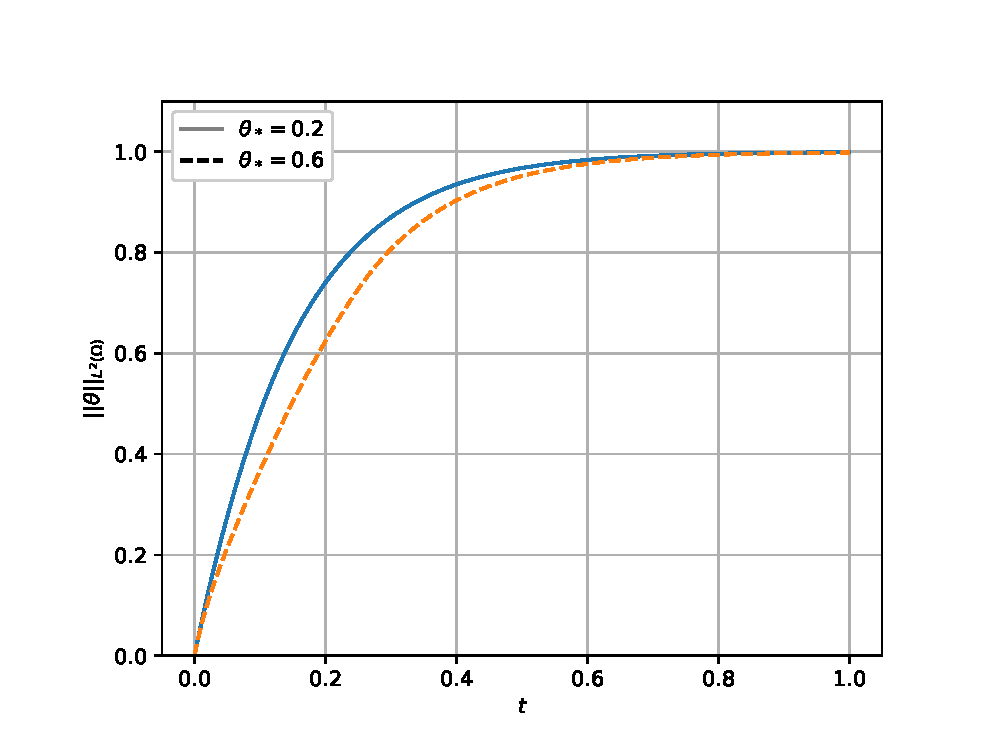
\includegraphics[width=1\linewidth]{additional/3/theta_dyn_star} \\ а) Первый эксперимент
%        \end{minipage}
%        \hfill
%        \begin{minipage}[b][][b]{0.49\linewidth}
%            \centering
%            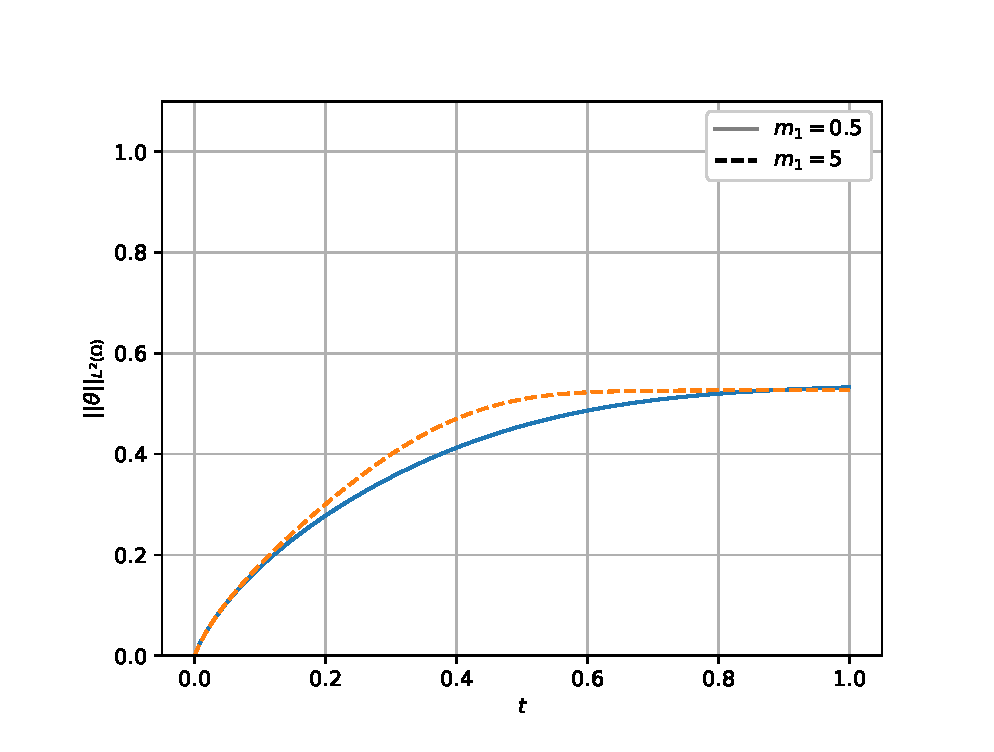
\includegraphics[width=1\linewidth]{additional/3/theta_dyn_m} \\ б) Второй эксперимент
%        \end{minipage}\label{fig:figure~~}
%    \end{figure}
%\end{frame}
%\note{
%    В рассмотренной модели коэффициент теплопроводности зависит от
%    неизвестной температуры (квазилинейность уравнения).
%    Это позволяет моделировать эффекты переноса энергии в областях с высокой температурой.
%    Разработанный комплекс программ позволяет оценить
%    влияние этого коэффициента на динамику темп поля.
%    температурного поля
%
%    Здесь показать анимацию.
%}
